% Generado por a_pdf.py desde reporte.md -- no editar a mano
\documentclass[11pt,a4paper]{article}
\usepackage[utf8]{inputenc}
\usepackage[T1]{fontenc}
\usepackage[spanish,mexico]{babel}
\usepackage{graphicx}
\usepackage[margin=2.5cm]{geometry}
\usepackage{amsmath}
\usepackage{booktabs}
\usepackage{tabularx}
\usepackage{array}
\usepackage{fvextra}
\usepackage{float}
\usepackage{setspace}
\usepackage{parskip}
\usepackage{fancyhdr}
\usepackage{textcomp}
\usepackage[hidelinks]{hyperref}

\onehalfspacing
\setlength{\parskip}{6pt}
\sloppy
\setlength{\emergencystretch}{3em}
\setlength{\headheight}{40pt}
\pagestyle{fancy}
\fancyhf{}
\fancyhead[L]{\includegraphics[width=1cm]{/home/yovick/repos/UAZ-IEI/Assets/UIE.png}}
\fancyhead[R]{\small Comunicaciones Inalámbricas}
\fancyfoot[C]{\thepage}
\renewcommand{\headrulewidth}{0.4pt}

\begin{document}

% ---------------------------- PORTADA -----------------------
\begin{titlepage}
  \thispagestyle{empty}
  \begin{center}
    \vspace*{1cm}
    \includegraphics[width=4.5cm]{/home/yovick/repos/UAZ-IEI/Assets/uaz.png}
    \vspace{0.8cm}

    {\large Universidad Autónoma de Zacatecas}\\[4pt]
    {\large Unidad Académica de Ingeniería Eléctrica}\\[4pt]
    {\normalsize Ingeniería Electrónica Industrial con especialidad en Telecomunicaciones}

    \vspace{1.8cm}
    {\LARGE\bfseries Práctica 2}\\[10pt]
    {\Large\bfseries Medición experimental de pérdidas por trayectoria (path loss)}
  \end{center}

  \vspace{2.2cm}
  \begin{center}
    \begin{tabular}{rl}
      \textbf{Materia:} & Comunicaciones Inalámbricas\\
      \textbf{Docente:} & Dr. Víktor Iván Rodríguez Abdalá\\
      \textbf{Alumno:}  & Arnold Yovick Ríos Zaldívar\\
      \textbf{Fecha:}   & Octubre de 2026\\
    \end{tabular}
  \end{center}
  \vfill
\end{titlepage}

\textbf{Equipo:} RTL-SDR (\texttt{RTL2832U} + tuner \texttt{R820T}), antena telescópica; transmisor LoRa/ISM a 433.9 MHz (pendiente de entrega)

\textbf{Script:} \texttt{practica2.py} (Python; en este repo el análisis se hace en Python en lugar de MATLAB)

\section{Objetivo}

Caracterizar experimentalmente la atenuación de una señal inalámbrica en función de la distancia entre transmisor y receptor, estimando por mínimos cuadrados el exponente de pérdidas $n$ del modelo logarítmico de propagación para el entorno analizado, y compararlo con los valores típicos reportados en la literatura.

\section{Fundamento teórico}

La potencia recibida a una distancia $d$ se modela con el \textbf{modelo logarítmico de pérdidas por trayectoria}:

\[
PL(d)\,[\text{dB}] = PL(d_0) + 10\,n\,\log_{10}\!\left(\frac{d}{d_0}\right) + X_\sigma
\]

o, en términos de potencia recibida con referencia a 1 m ($P_0 = P(1\,\text{m})$):

\[
P(d)\,[\text{dB}] = P_0 - 10\,n\,\log_{10}(d) + X_\sigma
\]

donde $n$ es el exponente de pérdidas y $X_\sigma \sim \mathcal{N}(0, \sigma^2)$ es el \emph{shadowing} log-normal (fluctuaciones lentas por obstáculos). Valores típicos:

\begin{tabularx}{\linewidth}{@{}*{2}{>{\raggedright\arraybackslash}X}@{}}
\toprule
Entorno & $n$ \\
\midrule
Espacio libre & 2.0 \\
Exterior urbano & 2.7 -- 3.5 \\
Interior oficinas & 3.0 -- 5.0 \\
Interior con obstáculos & 4.0 -- 6.0 \\
\bottomrule
\end{tabularx}

La potencia de cada bloque IQ se estima como $P(k)=\frac{1}{N}\sum_{i=0}^{N-1}|x[i]|^2$ y el nivel en dB como $P_{dB}=10\log_{10}\!\left(\overline{P}\right)$.

El ajuste por mínimos cuadrados de $P_{dB}$ contra $x=\log_{10}(d)$ es una recta $P_{dB}\approx a\,x+b$, de modo que

\[
n = -\frac{a}{10}, \qquad b = P_0 \text{ (intercepto en } d_0=1\,\text{m}), \qquad
R^2 = 1-\frac{\sum r_i^2}{\sum (P_i-\bar P)^2}
\]

\section{Desarrollo experimental}

\subsection{Configuración del receptor}

\begin{tabularx}{\linewidth}{@{}*{2}{>{\raggedright\arraybackslash}X}@{}}
\toprule
Parámetro & Valor \\
\midrule
Frecuencia central & \textbf{433.9 MHz} (banda ISM, frecuencia del nodo transmisor) \\
Sample rate & \textbf{2.4 MHz} \\
Muestras por medición & un bloque IQ de 131 072 muestras (\texttt{vivo.Fuente.ultimo}) \\
Mediciones por distancia & las que se registren con \texttt{ESPACIO} (10 en el procedimiento) \\
Ganancias & \textbf{auto calibrada}: mayor ganancia del R820T sin recorte del ADC (\texttt{comun.fijar\_ganancia}) \\
Distancias & \textbf{1, 2, 5, 10, 15 y 20 m} (\texttt{--distancias}) \\
Captura & asíncrona (\texttt{vivo.Fuente}), sin pérdida de muestras \\
\bottomrule
\end{tabularx}

\subsection{Procedimiento}

\begin{enumerate}
  \item Conectar el RTL-SDR a la PC y el transmisor LoRa a una fuente estable; fijar el transmisor en una posición y altura constantes.
  \item Ejecutar \texttt{python3 practica2.py -f 433.9e6}, que abre una sola ventana en vivo con espectro, cascada, la curva de potencia y sus residuales.
  \item En cada punto se pulsa la tecla de esa distancia (\texttt{1..6}) y \texttt{ESPACIO} para registrar una medición; se repite 10 veces por distancia.
  \item Cada medición es la potencia del último bloque IQ: $P=10\log_{10}\!\left(\text{mean}(|x|^2)\right)$; el ajuste de la recta se actualiza en vivo y calcula $n$, $R^2$ y los residuales.
  \item La tecla \texttt{s} guarda las mediciones en \texttt{datos/mediciones.csv}, el ajuste en \texttt{datos/resultados.json} y las figuras \texttt{figs/pathloss.png} y \texttt{figs/residuales.png}.
  \item Entorno de medición previsto: \textbf{pasillo del edificio E17-A} (interior con obstáculos), manteniendo visibilidad directa hacia el transmisor, misma orientación de antenas y sin tránsito de personas durante la captura.
\end{enumerate}

\begin{quote}
El dongle físico puede estar ocupado; la verificación del script se realizó con \texttt{--sim} (demo automática que recorre distancias y registra mediciones) y \texttt{--selftest}, que corren el mismo pipeline de ajuste sin hardware.
\end{quote}

\section{Código}

El script completo está en \texttt{practica2.py}. Fragmentos esenciales:

\begin{Verbatim}[breaklines=true,breakanywhere=true,fontsize=\small]
# Cada ESPACIO registra P = mean(|data|^2) del último bloque IQ
P[i].append(comun.potencia_dbfs(self.app.fuente.ultimo))   # P = 10*log10(mean(|x|^2))
self._actualizar_ajuste()                                   # recta, n y R2 en vivo

# Simulación log-normal: Pr(d) = P0 - 10*n*log10(d) + X_sigma
return p0 - 10.0 * n_real * np.log10(d)[:, None] + rng.normal(0, sigma, (d.size, nmed))

# Ajuste por mínimos cuadrados (equivalente a p = polyfit(log10(d), Pr, 1))
x = np.log10(d)
p = np.polyfit(x, Pr_dB, 1)                        # p = [pendiente, intercepto]
n = -p[0] / 10.0                                   # n = -p(1)/10
\end{Verbatim}

\section{Resultados}

\begin{quote}
\textbf{Los valores de esta sección provienen de la corrida de verificación por simulación (\texttt{python3 practica2.py --sim}), con $P_0=-40$ dB a 1 m, $n_{real}=3.2$ y $\sigma=4$ dB. Son datos sintéticos de verificación y se reemplazarán por los de la corrida real cuando llegue el transmisor LoRa.}
\end{quote}

\begin{tabularx}{\linewidth}{@{}*{3}{>{\raggedright\arraybackslash}X}@{}}
\toprule
Distancia (m) & Potencia (dB) & Observaciones ($\sigma$ de los 10 bloques) \\
\midrule
1 & $-$39.66 & 2.96 dB \\
2 & $-$51.44 & 3.48 dB \\
5 & $-$62.36 & 2.81 dB \\
10 & $-$71.51 & 2.74 dB \\
15 & $-$74.09 & 3.91 dB \\
20 & $-$82.36 & 3.10 dB \\
\bottomrule
\end{tabularx}

\begin{tabularx}{\linewidth}{@{}*{2}{>{\raggedright\arraybackslash}X}@{}}
\toprule
Parámetro del ajuste & Valor \\
\midrule
Exponente de pérdidas estimado & \textbf{n = 3.063} \\
Intercepto $P_0$ (a 1 m) & \textbf{$-$40.71 dB} \\
Coeficiente de determinación & \textbf{R$^2$ = 0.9890} \\
Desviación estándar de residuales & \textbf{1.51 dB} \\
\bottomrule
\end{tabularx}

\begin{center}
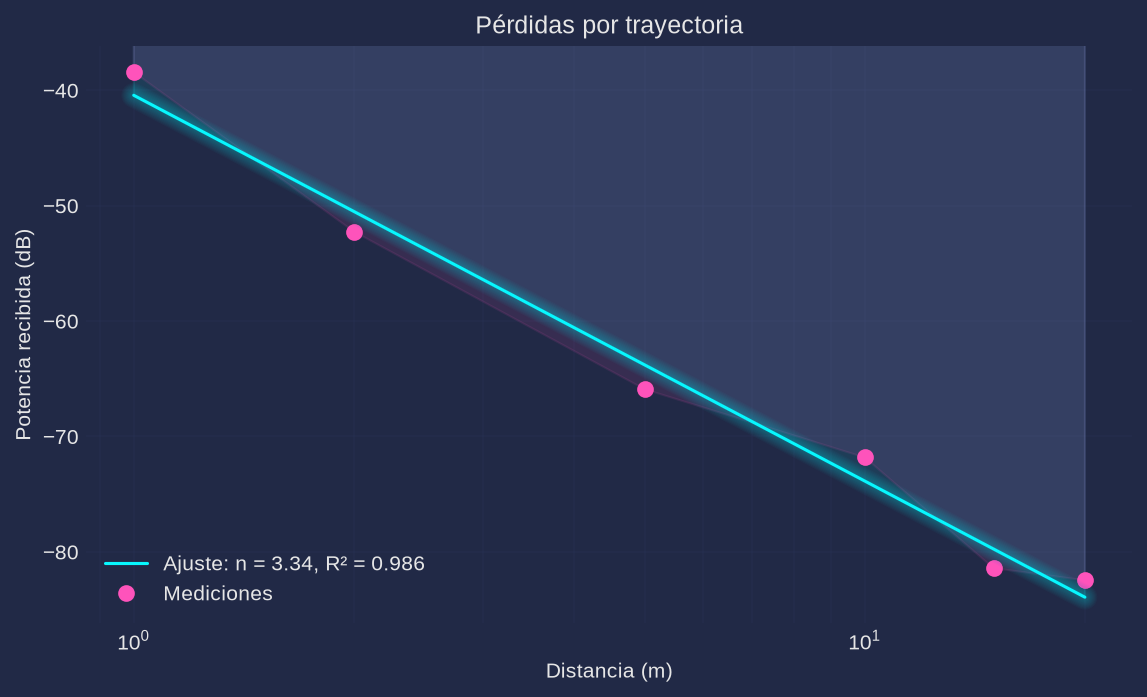
\includegraphics[width=0.9\linewidth]{figs/pathloss.png}\\[2pt]
{\small Pérdidas por trayectoria}
\end{center}

\begin{center}
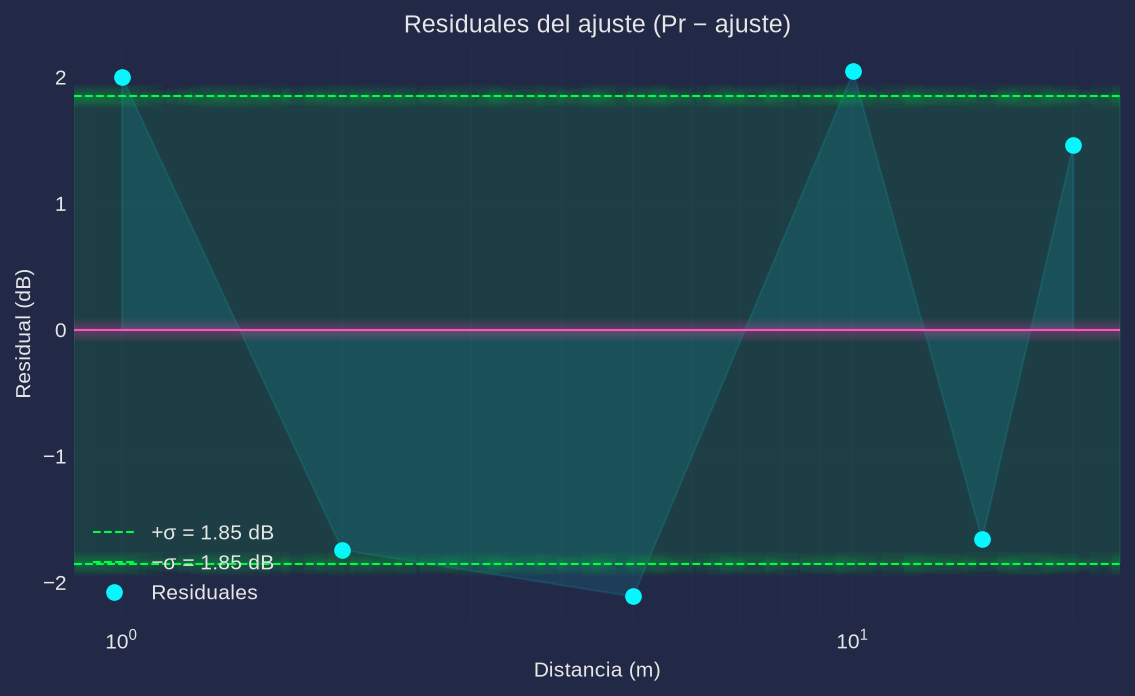
\includegraphics[width=0.9\linewidth]{figs/residuales.png}\\[2pt]
{\small Residuales del ajuste}
\end{center}

\section{Análisis de resultados}

\begin{itemize}
  \item La potencia decrece monótonamente con la distancia, como predice el modelo, y el ajuste logarítmico es excelente ($R^2=0.9890$).
  \item El exponente estimado $n=3.063$ difiere en solo $0.14$ del valor verdadero de la simulación ($n_{real}=3.2$). Comparado con la tabla de valores típicos, cae en el rango de \textbf{exterior urbano (2.7--3.5)} y en el extremo bajo de \textbf{interior de oficinas (3.0--5.0)}, lo que es consistente con un enlace con visibilidad directa y obstáculos moderados.
  \item El intercepto ajustado ($-40.71$ dB) reproduce el valor de referencia $P_0=-40$ dB con un error de 0.71 dB, absorbido por el shadowing.
  \item Los residuales no muestran una tendencia sistemática con la distancia y su desviación (1.51 dB) es compatible con el shadowing del generador: al promediar 10 bloques independientes, $\sigma_{\text{res}}\approx \sigma/\sqrt{10}=4/3.16\approx 1.27$ dB, del mismo orden que el valor medido. Esto confirma que promediar bloques reduce la varianza sin sesgar la pendiente.
  \item La dispersión por bloque ($\sigma$ entre 2.7 y 3.9 dB) evidencia el shadowing log-normal del canal: si se usara una sola captura por punto, la recta ajustada tendría mucha mayor incertidumbre.
  \item El entorno representado por estos parámetros es un canal con propagación cercana a la de espacio libre más atenuación moderada: en la corrida real en el pasillo E17-A se espera un $n$ mayor si predominan paredes y mobiliario, o menor si el efecto guía del pasillo domina.
\end{itemize}

\section{Cuestionario}

\begin{enumerate}
  \item \textbf{¿Qué representa físicamente el exponente de pérdidas?} Es la pendiente (normalizada) de la potencia recibida en dB por década de distancia; indica qué tan rápido decae la señal. Físicamente resume el mecanismo de propagación dominante: $n=2$ corresponde a la expansión esférica en espacio libre; valores mayores reflejan pérdida adicional por reflexión, difracción, dispersión y absorción de obstáculos. Cada 10 unidades de $n$ la potencia cae 100 dB por década.
\end{enumerate}

\begin{enumerate}
  \item \textbf{¿Por qué el valor de $n$ cambia según el entorno?} Porque cambian los mecanismos de propagación: en campo abierto domina la expansión en espacio libre ($n\approx2$); en la ciudad y en interiores se suman reflexiones en paredes y suelo, difracción en esquinas y absorción en muros, muebles y personas, que incrementan la atenuación media y por tanto $n$. También influyen la frecuencia, la altura y ganancia de las antenas y la presencia de guías de onda naturales (pasillos).
\end{enumerate}

\begin{enumerate}
  \item \textbf{¿Qué diferencias existen entre espacio libre y un entorno interior?} En espacio libre no hay obstáculos ni multitrayecto: la potencia decae de forma determinista con $n=2$ según Friis. En interiores hay multitrayecto (reflexiones, dispersión), sombras por muros y mobiliario, y desvanecimiento espacial/temporal, por lo que $n$ sube a 3--5 en oficinas y 4--6 con obstáculos, y aparece el shadowing log-normal. Además, en un pasillo el efecto guía puede hacer que $n$ baje incluso por debajo de 2 si las reflexiones laterales concentran energía hacia el receptor.
\end{enumerate}

\begin{enumerate}
  \item \textbf{¿Por qué es necesario realizar múltiples mediciones en cada punto?} Porque el canal es aleatorio: una sola captura incluye desvanecimiento de pequeña escala y ruido, y no representa la potencia media local. Promediar $N_{med}=10$ bloques independientes reduce la varianza del estimador aproximadamente en un factor $N_{med}$ y permite estimar la dispersión (shadowing) para cuantificar la incertidumbre del ajuste. También ayuda a detectar inestabilidad del transmisor o interferencias intermitentes.
\end{enumerate}

\begin{enumerate}
  \item \textbf{¿Qué factores limitan la precisión del experimento?} La falta de calibración absoluta del receptor (las potencias son dBFS, relativas al ADC, no dBm) y su rango dinámico de 8 bits; la ganancia automática puede cambiar entre capturas; el multitrayecto y el shadowing; la estabilidad y orientación de las antenas del transmisor y receptor; la incertidumbre en la colocación exacta de las distancias; el tránsito de personas o cambios del entorno durante las mediciones; y el reducido número de puntos de distancia (seis), que da pocos grados de libertad al ajuste.
\end{enumerate}

\section{Conclusiones}

Se implementó el pipeline completo de medición de pérdidas por trayectoria: registro de 10 mediciones por distancia con la tecla \texttt{ESPACIO}, cálculo de potencia, ajuste por mínimos cuadrados de $P_{dB}$ contra $\log_{10}(d)$, estimación de $n$, $R^2$ y residuales, guardado de CSV/JSON y generación de figuras con \texttt{s}. La corrida de verificación \texttt{--sim} (sin hardware) recuperó $n=3.063$ frente al valor nominal $n_{real}=3.2$ ($R^2=0.9890$, residuales de 1.51 dB, consistente con el shadowing promediado), lo que valida el procedimiento. La corrida real queda preparada para ejecutarse con \texttt{python3 practica2.py} cuando llegue el transmisor LoRa, y sus datos reemplazarán a los de la tabla anterior.

\end{document}
